\documentclass[a4paper,12pt]{article}
\usepackage[swedish]{babel}
\usepackage[utf8]{inputenc}
\usepackage{amsmath, amsthm, amssymb}
\usepackage{graphicx}
\usepackage[a4paper,includeheadfoot,margin=2.54cm]{geometry}
\begin{document}

\section{Dugga 2 - Fråga 3}
Här ska ett logiskt uttryck $X$ analyseras. Kolumnen under $X$ ska i appen ges
som en vektor.
\begin{center}
\begin{tabular}{ ccc | c } 
    $p$ & $q$ & $r$ & $X$ \\ 
    \hline
    0 & 0 & 0 & ? \\ 
    0 & 0 & 1 & ? \\ 
    0 & 1 & 0 & ? \\ 
    0 & 1 & 1 & ? \\ 
    1 & 0 & 0 & ? \\ 
    1 & 0 & 1 & ? \\ 
    1 & 1 & 0 & ? \\ 
    1 & 1 & 1 & ? \\ 
\end{tabular}
\end{center}
\subsection*{Fråga}
Bestäm en sanningsvärdestabell enligt ovan då $X$ är
\begin{displaymath}
    \left(\neg p \wedge r\right) \wedge \left(\left(r \rightarrow q\right) \leftrightarrow \left(p \rightarrow r\right)\right).
\end{displaymath}
och om vi sätter in det i värdestabell
\begin{center}
\begin{tabular}{ ccc | c | ccc | c }
    $p$ & $q$ & $r$ & $\neg p$ & $\neg p \wedge r$ & $r \rightarrow q$ & $p
    \rightarrow r$ & Ekvivalens $\leftrightarrow$ \\ 
    \hline
    0 & 0 & 0 & 1 & 0 & 1 & 1 & 1 \\ 
    0 & 0 & 1 & 1 & 1 & 0 & 1 & 0 \\ 
    0 & 1 & 0 & 1 & 0 & 1 & 1 & 1 \\ 
    0 & 1 & 1 & 1 & 1 & 1 & 1 & 1 \\ 
    1 & 0 & 0 & 0 & 0 & 1 & 0 & 0 \\ 
    1 & 0 & 1 & 0 & 0 & 0 & 1 & 0 \\ 
    1 & 1 & 0 & 0 & 0 & 1 & 0 & 0 \\ 
    1 & 1 & 1 & 0 & 0 & 1 & 1 & 1 \\ 
\end{tabular}
\end{center}
mitt svar är då att $X$ är
\begin{center}
\begin{tabular}{ cccc | c }
    $\neg p \wedge r$ & $r \rightarrow q$ & $p
    \rightarrow r$ & Ekvivalens $\leftrightarrow$ & $X$ \\ 
    \hline
    0 & 1 & 1 & 1 & 0 \\ 
    1 & 0 & 1 & 0 & 0 \\ 
    0 & 1 & 1 & 1 & 0 \\ 
    1 & 1 & 1 & 1 & 1 \\ 
    0 & 1 & 0 & 0 & 0 \\ 
    0 & 0 & 1 & 0 & 0 \\ 
    0 & 1 & 0 & 0 & 0 \\ 
    0 & 1 & 1 & 1 & 0 \\
\end{tabular}
\end{center}
\begin{center}
    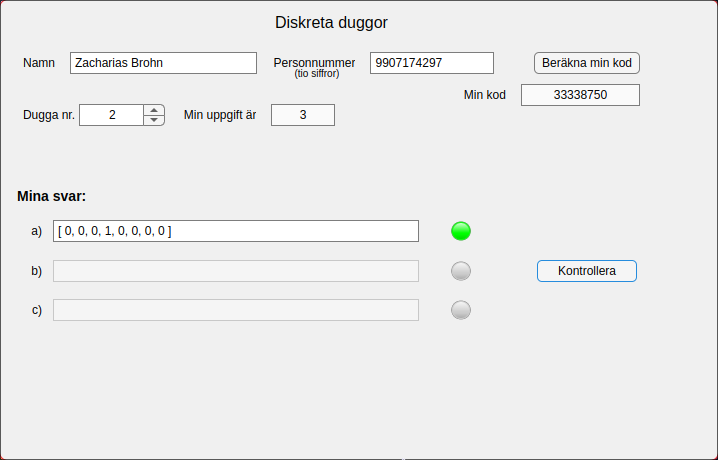
\includegraphics[width=15cm]{iPpJZWB.png}
\end{center}
\end{document}